\subsubsection{Endschalter}
Für den Ballvorschub sind elektronische und kontaktlose Endschalter
eingesetzt, welche das Erreichen der Endposition erkennen für den
Ballvorschub. Dies ist eine wichtige Schutzmassnahme, da diese
nicht in den Anschlag gehen darf, was den Motor des Vorschubs
überansprucht.

Für diese Funktion sind magnetisch getriggerte Hall-Effekt-Schalter
eingesetzt vom Typ AH180N von Diodes Incorporated. Hierzu sind eigens
etstellte Platinen der PREN-ET Subgruppe DC im Einsatz.

\begin{figure}[h!]
	\centering
	\begin{subfigure}[b]{0.45\textwidth}
		\centering
		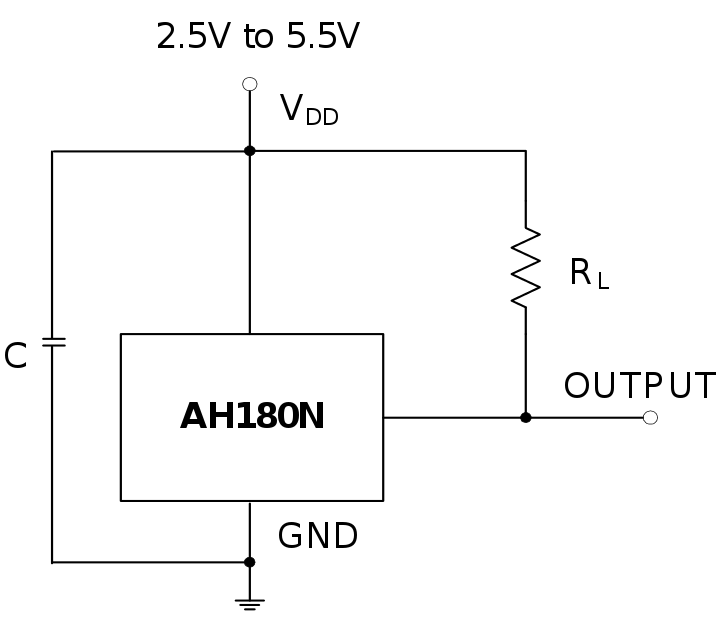
\includegraphics[width=1\textwidth]{../../fig/et/ah180n.png}
		\caption{Typical Application AH180N}
	\end{subfigure}
	\begin{subfigure}[b]{0.45\textwidth}
		\centering
		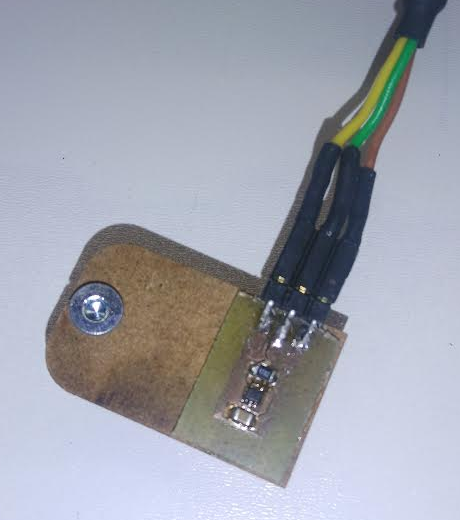
\includegraphics[width=1\textwidth]{../../fig/et/sensor_pcb.png}
		\caption{Endschalter-Platine}
	\end{subfigure}
	\caption{Endschalter für den Ballvorschub}
\end{figure}

Die Hall-Effekt-Schalter werden mit der vom Freedomboard zur Verfügung
gestellten 3.3 Volt Speisung betrieben. Da die Ausgangsstufe des Sensors
als Open-Collector implementiert ist, kann so das 3.3 Volt Signal direkt
auf das Freedomboard zurückgeführt und verarbeitet werden. 
%
Die Signale der Endschalter sind als Interruptquellen in der Firmware des
Freedomboard implementiert und reagieren auf fallende Signalflanken. Da
der Hall-Effekt-Schalter eine Hysterese besitzt, gibt es ein sauberes
Signal an den Eingängen ohne Prellen.
%
Die Firmware bindet die Interrupts direkt an den Ballvorschub in der Weise,
dass der Motor unverzüglich abgestellt wird und präventiv die Drehrichtung
geändert wird. Die Änderung der Drehrichtung richtet sich nach dem
aktivierten Sensor. So wird die Drehrichtung auf Abwärts gestellt
falls der obere Endschalter ausschlägt und umgekehrt beim unteren.
%
Die Zustände der Endschalter können über die Statusanzeige vom DC-Motor
eingesehen werden auf der Kommandozeile. Die Quittierung der Sensoren
erfolgt per Einschalten des DC-Motors.

Die Firmware auf dem Freedomboard bietet noch zwei Besonderheiten im
Zusammenhang mit den Endschaltern. Zum einen sind beide per Default nach
einem Reset als aktiv gesetzt und zum anderen wird ein ausgeschlagener
Endschalter den Zustand der RGB-LED auf dem Freedomboard orange färben,
sonst ist diese grün.
